\chapter{Introduction and Context}
\label{Chapter1}

\section{Introduction}

\section{Context}

Before explaining the main problem which this project is about, \emph{Pseudo-Boolean Minimization}, it necessary to do a quick introduction to a much wider topic.\\

\textbf{Boolean satisfiability problems} \textit{(SAT from now on)} is the problem of finding a model\footnote{An interpretation which satisfies the formula.} for a \emph{Boolean Formula} (BF from now on). In other words, it is the result of evaluating the \emph{BF} after replacing its variables for \emph{true} or \emph{false}. 
\\
\emph{SAT} is widely used in Computer Science because it was the first problem proved to be NP-Complete\cite{Cook1971}\footnote{NP and NP-Hard.} which allowed a lot of NP\footnote{Nondeterministic polynomial time.} problems be reduced to it.

\subsubsection{What is a Pseudo-Boolean Formula?}
In propositional logic, a \emph{BF} is defined as following\cite{Lpo}:\\
Let $P$ be a set of predicate symbols like $p,q,r,...$
\begin{itemize}
	\item All predicate symbol of $P$ is a formula.
	\item If $F$ and $G$ are formulae, then $(F \land G)$ and $(F \lor G)$ are formulae too.
	\item If $F$ is a formula, then $(\neg F)$ is a formula.
	\item Nothing else is a formula.
\end{itemize}
This representation has some limitations because it can only express properties which are \emph{true} or \emph{false}.\\

\emph{Pseudo-Boolean Formulas} are functions of the form $f:B^n \rightarrow \mathbb{R}$. For example, the following formula is a \emph{Pseudo-Boolean Formula} (PBF from now on): $3x+5y$. Therefore, \emph{BF} are a special case of \emph{PBF} where the domain is $d=\{0,1\}$.\\

%TODO: potser explicar que son cardinality constraints


\subsubsection{Pseudo-Boolean formulae minimization}
\emph{PBF minimization} is a well known NP-Hard\footnote{NP-Hard: at least as hard as the hardest problems in NP \href{https://en.wikipedia.org/wiki/NP-hardness}{(more)}} problem. \\
It does the following:\\
Given some \emph{PB Constraints} of the form $\sum_{i=1}^{n} x_{i}w_{i} \leq k$, where $w_{i},k \in \mathbb{I}$ and $x_{i} \in \{0,1\}$, and a cost function , the goal is minimize it  $min(a_{1}x{1} + ... + a_{n}x_{n})$ in a way that all the restrictions are satisfied.\\

There is a big research in this field, more specifically in encoding \emph{PBF} into \emph{CNF}. In this paper, Hölldobler, Manthey, Steinke\cite{Holldobler}, some relevant \emph{PBF} into \emph{SAT} encodings are explained and a new one is proposed. One of the authors of this paper, Steinke, is also the author of \emph{PBLib}.  

\section{Background}

During the past semester (Q1 2017/2018), under the supervision of \href{https://www.cs.upc.edu/~jordicf/}{Dr. Jordi Cortadella}, I had been developing a C++ library.\\
This tool allows the users to represent \emph{BF} in a C++ program in an intuitive way, do operations between them and convert them into \emph{Binary Decision Diagrams} (BDD from now on). However, the main functionality of this library is the conversion from a \emph{BF} to \emph{CNF}.  \\
As previously explained, \emph{CNF} is a particular type of a \emph{BF}, a conjunction of disjunctions. \emph{CNF} is an important format because it is the standard input for \emph{SAT Solvers}\ref{A.1}.\\
As shown in this paper, \emph{Mitchell, Selman, and Levesque\cite{Mitchell}}, there is a correlation between the number of variables, the number of clauses and the hardness of solving the \emph{CNF}.
\begin{center}
	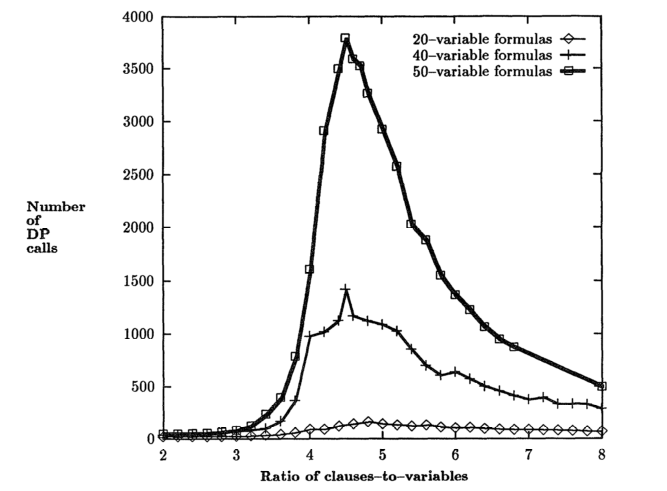
\includegraphics[width=1\textwidth]{Figures/GraphMitchellSelmanLevesque.png}
	\captionof{figure}{Median number of recursive DP calls for Random 3-SAT formulas, as a function of the ratio of clauses-to-variables. \\Extracted from Mitchell, Selman, and Levesque\cite{Mitchell}}
\end{center}
Therefore, an improvement of the input \emph{CNF} of the \emph{SAT Solver} can reduce a lot the hardness of the problem. \\
This is the main goal of the library, try to reduce the size of the final \emph{CNF} resulting from applying different converting methods on the original BF.

\section{State-of-the-art}

In this section, previous projects are discussed. \\
The first one is \href{http://tools.computational-logic.org/content/pblib.php}{PBLib}. PBLib is a C++ toolkit for encoding \emph{PB Constraints} into \emph{CNF}.\\
As explained in \emph{Steinke}\cite{Steinke2015}, PBLib implements a lot of encodings:
\begin{center}
	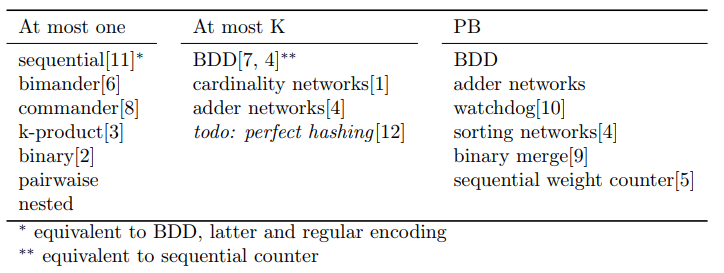
\includegraphics[width=1\textwidth]{Figures/PBLibEncodings.png}
	\captionof{figure}{PBLib implemented encodings\\Extracted from Steinke\cite{Steinke2015}}
\end{center}
PBLib does not only implement these encodings, the most interesting thing is that it can decide which encoder provides the most effective translation.\\
It is very hard to compete on this aspect against PBLib, but it is not very user-friendly. For this reason, on of the goals of this project is to add a layer between the user and PBLib to simplify how the user declares the \emph{PB Constraints}.\\\\

The second project we will talk about is the explained in the \emph{Background section}. This project adds a new encoding for \emph{BF} which can be extended to \emph{PB Constraints}. This encoding will be studied and if it achieves good metrics it will be implemented to \emph{PB Constraints}


\section{Motivations}

\href{https://www.fib.upc.edu/en/studies/bachelors-degrees/bachelor-degree-informatics-engineering/curriculum/syllabus/LI}{Informatics Logic} is taught in this\footnote{\href{https://www.fib.upc.edu/en/}{Facultat Informàtica de Barcelona}} faculty. In that course, I realized how important is \emph{logic} through its lecturer, \href{http://www.lsi.upc.es/~roberto/}{Dr. Robert Nieuwenhuis}, and its activities. \\

In the first coursework, we had to code a \emph{SAT Solver} which used \emph{Unit Propagation}.
%\ref{A.2}. 
With this activity, I comprehended how hard and substantial is the study of \emph{logic} and all its context. For example, how \emph{logic} is used in Artificial Intelligence and Planners.\\

When the time of deciding the \emph{TFG} arrived, I contacted my actual supervisor, \href{https://www.cs.upc.edu/~jordicf/}{Dr. Jordi Cortadella}, and he proposed me some topics and ideas. Finally, we agreed on doing this project. \\

The motivation for this project is trying to deepen into the topic and contribute on it.

\section{Stakeholders}

In this section, the Stakeholders of the project are defined. Stakeholders are entities which are affected, directly or indirectly, by the solution developed in this project. 
\subsection{Target audience}
This tools targets all the entities (researchers, companies, \ldots) which work with \emph{PB minimization} and use \emph{SAT Solvers}.
\subsection{Users}
The users will be C++ programmers due this tool is developed in this language.
\subsection{Beneficiaries}
All those entities which work with \emph{PB minimization}. For example AI, SAT Solvers, Planners, \ldots